\documentclass[a4paper]{article}
\usepackage[top=0in, bottom=0.20in, left=0.40in, right=0.40in]{geometry}
\usepackage[english]{babel}
\usepackage{enumitem}
\usepackage{hyperref}
\usepackage{xcolor}
\usepackage{titlesec}
\usepackage{graphicx}
\usepackage{tikz}

\definecolor{graytext}{HTML}{666666}
\hypersetup{hidelinks}

% Section formatting - Large bold text without underlines
\titleformat{\section}{\LARGE\bfseries}{}{0em}{}
\titlespacing*{\section}{0pt}{-4pt}{-2pt}

% List formatting - Spacings for readability
\setlist[itemize]{noitemsep, topsep=0.7pt, partopsep=0pt, parsep=0pt, itemsep=0pt, leftmargin=1.5em, labelsep=1.1em, after=\vspace{0.02in}}

% Set Carlito font
\usepackage{fontspec}
\setmainfont{Carlito}

\pagestyle{empty}
\renewcommand{\baselinestretch}{1.0}
\setlength{\parindent}{0pt}

% Helper for bigger names in <name><institution><date> structure
\newcommand{\entrytitle}[1]{{\fontsize{12pt}{13.2pt}\selectfont\textbf{#1}}}

\begin{document}
\fontsize{10.5pt}{11.8pt}\selectfont

\begin{tikzpicture}[remember picture, overlay]
    \node[anchor=north east, xshift=-0.35in, yshift=-0.06in] at (current page.north east) {
        \setlength{\fboxsep}{0pt}
        \setlength{\fboxrule}{0.5pt}
        {\color{graytext}\fbox{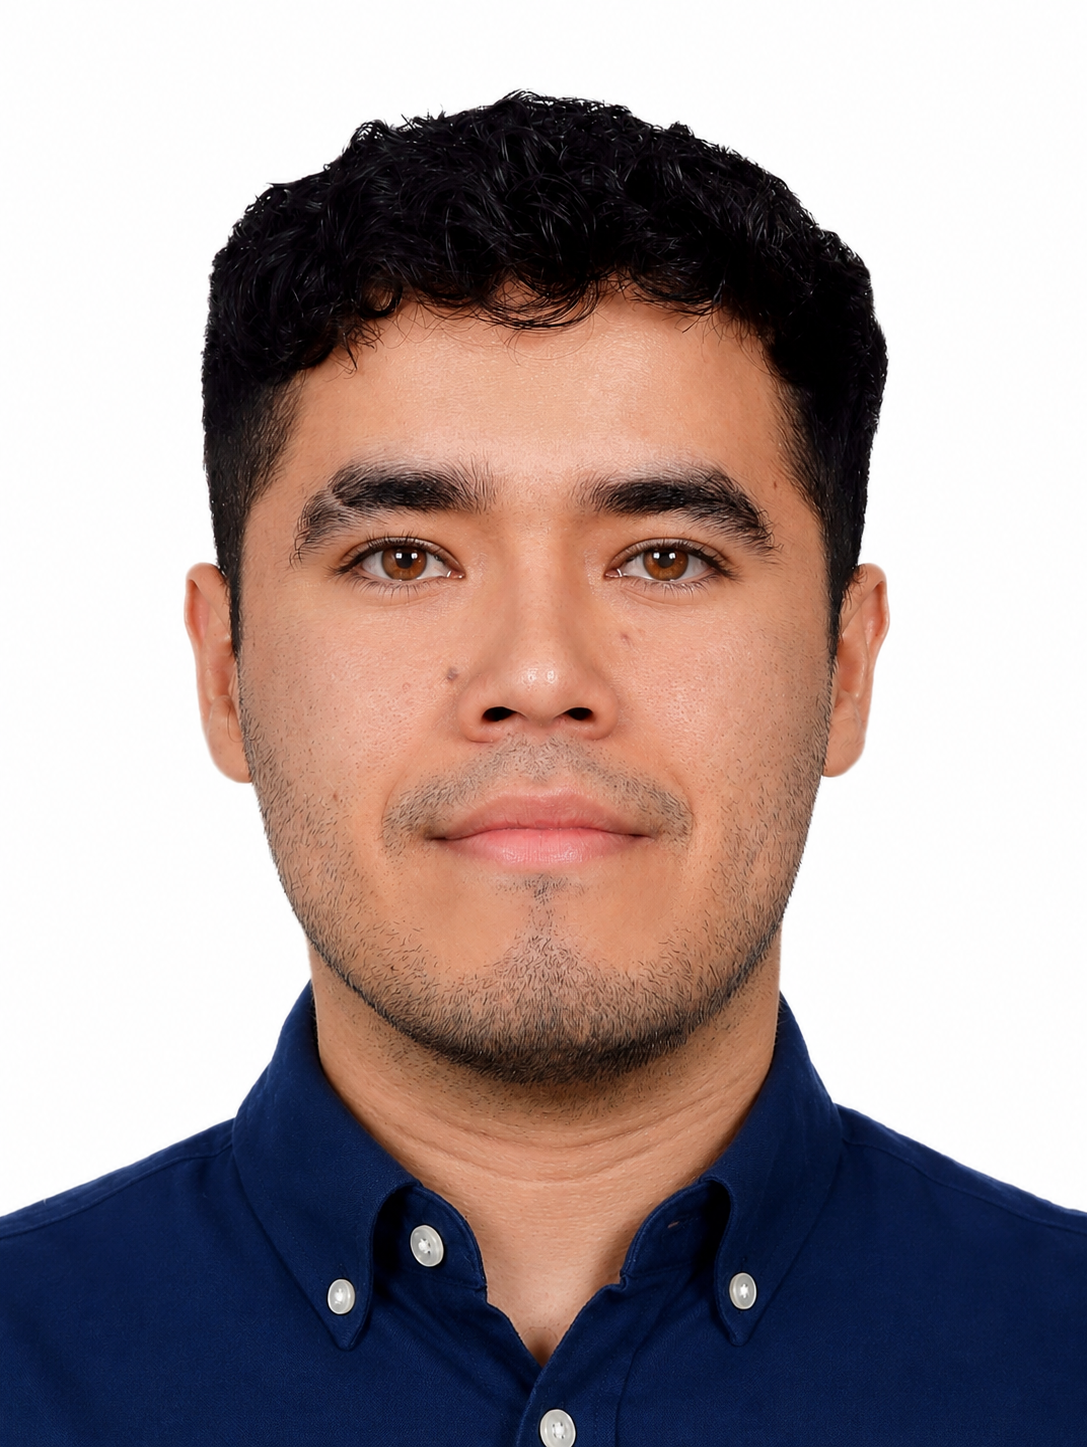
\includegraphics[width=2cm, keepaspectratio]{pfp.png}}}
    };
\end{tikzpicture}

\begin{center}
    {\fontsize{18pt}{20.6pt}\selectfont \textbf{Eduardo Venegas Hernandez}} \\[0.08cm]
    \small Data \& AI Engineer \textbar{} Munich, Germany \\[0.04cm]
    \small \href{https://lalovene.netlify.app}{lalovene.netlify.app} \textbar{} \href{https://www.linkedin.com/in/eduardo-venegas/}{linkedin.com/in/eduardo-venegas} \textbar{} \href{https://github.com/LaloVene}{github.com/LaloVene}
\end{center}

\vspace{-0.10cm}

\section*{EDUCATION}

\entrytitle{MSc. Data Science and Artificial Intelligence} {\small \textcolor{graytext}{Universität des Saarlandes} \hfill \textcolor{graytext}{Saarbrücken, Germany \quad \textit{10/2024 - 09/2026}}}
\begin{itemize}
    \item Coursing: \textit{Statistics}, \textit{ML Cybersecurity}, \textit{NLP}, \textit{Machine Translation}, \textit{Image Processing \& Computer Vision}.
    \item \textbf{Thesis (Seminar Grade 1.0)}: Evaluating \textbf{Multi-Turn Agentic RAG Systems} (In collaboration with \textbf{BMW} \& \textbf{DFKI}).
\end{itemize}

\vspace{0.1cm}
\entrytitle{BSc. Computer Science} {\small \textcolor{graytext}{Tecnológico de Monterrey} \hfill \textcolor{graytext}{Guadalajara, Mexico \quad \textit{08/2019 - 12/2023}}}
\begin{itemize}
    \item \textit{ML}, \textit{Time series}, \textit{Algorithms \& Optimization}, \textit{Cloud Computing \& Distributed}, \textit{Vehicle User Interfaces}, \textit{PLC}.
\end{itemize}

\vspace{0.1cm}
\entrytitle{Computer Science Exchange Student} {\small \textcolor{graytext}{Universität Ulm} \hfill \textcolor{graytext}{Ulm, Germany \quad \textit{10/2022 - 09/2023}}}
\begin{itemize}
    \item Full scholarship recipient from \textbf{DAAD}. \textit{Computer Vision II}, \textit{Autonomous Driving and Assistance Systems}, \textit{Statistics}.
\end{itemize}

\vspace{0.1cm}
\entrytitle{Technologist Degree in Automation and Robotics} {\small \textcolor{graytext}{CETI Colomos} \hfill \textcolor{graytext}{Guadalajara, Mexico \quad \textit{08/2015 - 06/2019}}}
\begin{itemize}
    \item Grade: 94.6 / 100. Five times best software engineering GPA. \textbf{60\% tuition scholarship due to academic merit}.
    \item \textit{Control Laboratory (I \& II)}, \textit{Industrial Robotics}, \textit{PLCs}, \textit{Digital Electronics}, \textit{Controllers Laboratory}, \textit{Sensor Systems}
\end{itemize}

\section*{SKILLS}

\textbf{AI \& Data:} PyTorch, LangGraph, LangChain, MLflow, RAG, Knowledge Graphs, MCP, Hugging Face, TensorFlow, Vector DB, SQL \\
\textbf{Software \& Frameworks:} Python, C/C++, TypeScript/JavaScript, FastAPI, Flask, Node.js, React, Next.js, Angular, Tauri \\
\textbf{Systems \& DevOps:} Linux, Docker, Kubernetes, CI/CD, AWS, Azure, Git, Grafana, MQTT, PLCs

\section*{WORK EXPERIENCE}

\entrytitle{Data \& AI Engineer Masterarbeit} {\small \textcolor{graytext}{BMW \& DFKI} \hfill \textcolor{graytext}{Munich, Germany \quad \textit{03/2026 - 09/2026}}}
\begin{itemize}
    \item Topic: Evaluating \textbf{Multi-Turn Agentic RAG Systems}: A \textbf{Synthetic Benchmark Generation} Approach.
    \item Architected an evaluation framework for \textbf{multi-turn tool-using Agentic RAG} systems enabling precise failure localization.
    \item Built a multi-turn synthetic benchmark pipeline that combines deterministic \textbf{task planning} with diverse user \textbf{personas}.
    \item Engineered an \textbf{unsupervised audit framework} for a \textbf{RAG system} across \textbf{4M unannotated} corporate records.
\end{itemize}

\vspace{0.1cm}
\entrytitle{AI Research Engineer Werkstudent} {\small \textcolor{graytext}{August-Wilhelm Scheer Institute} \hfill \textcolor{graytext}{Saarbrücken, Germany \quad \textit{10/2024 - 02/2026}}}
\begin{itemize}
    \item Designed and deployed a \textbf{KG-RAG} over unstructured technical documentation using \textbf{LangChain} and \textbf{HuggingFace}.
    \item Developed an \textbf{Autoencoder model} for real-time \textbf{anomaly detection} across \textbf{distributed devices} via \textbf{Federated Learning}.
\end{itemize}

\vspace{0.1cm}
\entrytitle{Big Data Platform Engineer} {\small \textcolor{graytext}{Oracle} \hfill \textcolor{graytext}{Guadalajara, Mexico \quad \textit{11/2023 - 10/2024}}}
\begin{itemize}
    \item Engineered \textbf{CI/CD testing pipelines} and deployment tools of \textbf{big data clusters} on \textbf{Oracle Cloud Infrastructure (OCI)}.
    \item Maintained \textbf{automation frameworks} within the \textbf{Big Data Service} team under \textbf{Oracle Analytics}.
\end{itemize}

\vspace{0.1cm}
\entrytitle{Data Science \& Analytics Intern} {\small \textcolor{graytext}{BMW Group} \hfill \textcolor{graytext}{Munich, Germany \quad \textit{03/2023 - 09/2023}}}
\begin{itemize}
    \item Developed a high-accuracy \textbf{anomaly detection algorithm} specialized in identifying external \textbf{battery replacements}.
    \item Engineered scalable \textbf{time-series data pipelines} using \textbf{PySpark} to process raw \textbf{vehicle telemetry} and \textbf{cloud logs}.
    \item Optimized \textbf{data flows}, resolving missing \textbf{database values} to increase \textbf{data reliability} and a 62\% increase in \textbf{service utilization}.
    \item Allowed adjusting \textbf{predictive model parameters} and receive real-time \textbf{system performance outputs}.
\end{itemize}

\vspace{0.1cm}
\entrytitle{AI \& DevOps Engineer} {\small \textcolor{graytext}{Xira} \hfill \textcolor{graytext}{Mexico City, Mexico \quad \textit{01/2022 - 04/2022}}}
\begin{itemize}
    \item Managed over \textbf{distributed server infrastructure}, established \textbf{service monitoring} and enhanced engineering processes.
    \item Built an \textbf{API management platform}, integrating payments and subscription systems using \textbf{NextJS}, \textbf{Stripe} and \textbf{Docker}.
\end{itemize}

\vspace{0.1cm}
\entrytitle{Production Engineer Fellow} {\small \textcolor{graytext}{Major League Hacking \& Meta} \hfill \textcolor{graytext}{New York, USA \quad \textit{06/2021 - 09/2021}}}
\begin{itemize}
    \item Selected internationally among 120 out of 20,000 applicants. Implemented \textbf{monitoring} with \textbf{Prometheus} and \textbf{Grafana}.
    \item Automated \textbf{CI/CD workflow} for efficient deployment to a production server using \textbf{Docker} in an \textbf{AWS EC2 instance}.
\end{itemize}

\vspace{0.1cm}
\entrytitle{Machine Learning \& Full Stack Engineer} {\small \textcolor{graytext}{Jiit Technologies} \hfill \textcolor{graytext}{Guadalajara, Mexico \quad \textit{10/2020 - 06/2021}}}
\begin{itemize}
    \item Designed a custom \textbf{sales forecasting} and \textbf{data analytics API pipeline} using \textbf{Flask}, \textbf{SciPy} and \textbf{Prophet}.
    \item Built an \textbf{ERP platform} to handle multi-module operations (inventory, logistics, and finance) utilizing \textbf{Angular}.
\end{itemize}

\section*{PROJECTS}

\entrytitle{VectorDrive-Route: Autonomous BEV Trajectory Planning} \hfill {\small \textcolor{graytext}{\textit{\href{https://github.com/LaloVene/vectordrive-route}{Github}}}}
\begin{itemize}
    \item Built a \textbf{PyTorch pipeline} using \textbf{nuScenes}, \textbf{ResNet} and \textbf{depth lifting} to map multi-camera feeds into a \textbf{Bird’s-Eye-View grid}.
    \item Designed a temporal \textbf{motion planning head} with \textbf{drivable-area} and \textbf{occupancy decoders} to generate safe paths.
\end{itemize}

\vspace{0.1cm}
\entrytitle{Daten-Mapping-Framework für die AAS} \hfill {\small \textcolor{graytext}{\textit{\href{https://doi.org/10.17560/atp.v68i5.2836}{DOI: 10.17560/atp.v68i5.2836}}}}
\begin{itemize}
    \item Developed a mapping framework from \textbf{schemas} to \textbf{Asset Administration Shell} to achieve interoperability in \textbf{Industry 4.0}.
    \item Designed a dual alignment strategy separating standard \textbf{relational tables} from \textbf{hierarchical assets}.
\end{itemize}

\vspace{0.1cm}
\entrytitle{See Your World} \hfill {\small \textcolor{graytext}{\textit{\href{https://github.com/LaloVene/Image-Captioning-Project}{Github}}}}
\begin{itemize}
    \item Crafted a hackathon award-winning app for the visually impaired, supporting 11 languages.
    \item Engineered \textbf{Image Captioning DL model} with \textbf{TensorFlow}, deployed using \textbf{Flask}, \textbf{Docker}, and \textbf{Google Cloud VM}.
\end{itemize}

\begin{minipage}[t]{0.62\textwidth}
\section*{CERTIFICATES}
\begin{itemize}
    \item \textbf{Mathematics for Data Science Specialization} {\small \textcolor{graytext}{HSE - 2021}}
    \item \textbf{Data Science Professional Certificate} {\small \textcolor{graytext}{Harvard - 2020}}
    \item \textbf{Python Data Science Professional Certificate} {\small \textcolor{graytext}{IBM - 2020}}
    \item \textbf{Deep Learning Professional Certificate} {\small \textcolor{graytext}{IBM - 2020}}
\end{itemize}
\end{minipage}
\hfill
\begin{minipage}[t]{0.33\textwidth}
\section*{LANGUAGES}
\begin{itemize}
    \item \textbf{Spanish:} Native
    \item \textbf{English:} C1
    \item \textbf{German:} C1
\end{itemize}
\end{minipage}

\end{document}
